\documentclass[]{article}
\usepackage{amsfonts}
\usepackage{amsmath}
\usepackage{amsthm}
\usepackage{amssymb}
\usepackage{mathrsfs}
\usepackage[numbers]{natbib}
\usepackage[fit]{truncate}
\usepackage{graphicx}
\usepackage{tkz-euclide}

\theoremstyle{plain}
\newtheorem{theorem}{Theorem}[section]
\newtheorem{corollary}[theorem]{Corollary}
\newtheorem{lemma}[theorem]{Lemma}
\newtheorem{claim}[theorem]{Claim}
\newtheorem{proposition}[theorem]{Proposition}
\newtheorem{question}{Question}
\newtheorem{conjecture}[theorem]{Conjecture}
\theoremstyle{definition}
\newtheorem{definition}[theorem]{Definition}
\newtheorem{example}[theorem]{Example}
\newtheorem{notation}[theorem]{Notation}
\newtheorem{exercise}[theorem]{Exercise}



%opening
\title{Analysis of Runge's Phenomenon using Chebyshev Nodes for Polynomial Interpolation}
\author{Casey Chesshir}

\begin{document}

\maketitle

\begin{abstract}
Suppose we want to interpolate data that closely resembles Runge's function. How should we do it? 
\end{abstract}

\section{Introduction}

We begin with a table of values.

\begin{tabular}{l*{6}{c}r}
x : & $x_0$ & $x_1$ & $x_2$ & $...$ & $x_{n-2}$  & $x_{n-1}$ & $x_n$ \\
\hline
y : & $y_0$ & $y_1$ & $y_2$ & $...$ & $y_{n-2}$  & $y_{n-1}$ & $y_n$ \\
\end{tabular}

\begin{definition}
Runge's Function $\cite{runge}$ will be denoted by R(x) = $\frac{1}{1+25x^2}$ 
\end{definition}


\begin{definition}
Interpolation polynomial $P(x)$ = $\sum_{i=0}^{n} (\frac{x-x_{i+1}}{x_i - x_{i+1}})y_i$

This polynomial interpolates exactly correctly for the given table of values. That is, $P(x_i) = y_i$ $\forall i \leq n$. For points $x$ such that $x_i < x < x_{i+1}$ for some $i$, that is, intermediate values between the given nodes, an approximation is attempted. 

\end{definition}

\begin{definition}
Nodes 

Nodes are points on the real line $x_0 ... x_n$ to be used for polynomial interpolation. These will be generated by choosing a step size $h = \frac{b-a}{n}$, where $a,b$ are endpoints of the closed interval to be interpolated, and $n$ is the number of nodes in that interval.  

$\{x_0, x_1, x_2, ..., x_{n-1}, x_n\} = \{a, a+2h, a+3h, ..., b - h, b\}$
\end{definition}

\begin{definition}
Chebyshev Nodes 

Chebyshev Nodes are also points on the real line $x_0 ... x_n$ but are generated using a different scheme from regular Nodes. Each $x_i$ for $0 \leq i \leq n$ is taken from equally spaced points on a semicircle projected above the interpolation interval. Interpolation polynomials generated using Chebyshev nodes will be denoted $P_c(x)$.

\includegraphics[scale=0.2]{semicircle.png} 

$\cite{book}$ above, a semicircle projected onto the interval [-5,5]
\newline 

Each $x_i$ can be derived graphically by solving the following triangle. 

$\theta_0 = \frac{180}{n}, \theta_i = \theta_{i-1} + \theta_0$  

$r =  \frac{b-a}{2}$ This is the radius of the semicircle. It is constant and does not vary with $i$. 

$midpoint = \frac{1}{2}(a+b)$ This is the midpoint of the interval $[a,b]$ and the center of the projected semicircle. 

$base_i = r\cdot\cos\theta_i$

$x_i = midpoint + base_i$

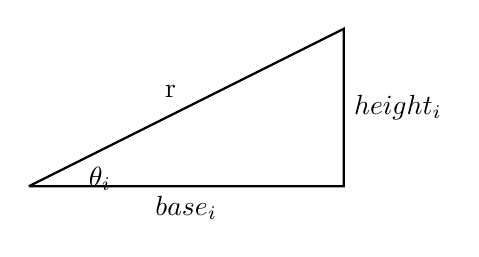
\begin{tikzpicture}[thick]
\draw(0,0) -- node[midway,below]{$base_i$} 
         (4,0) -- node[midway,right]{$height_i$}
         (4,2) -- node[midway,above left]{r}
         (0,0);
\hspace{.3in} {$\theta_i$};
\end{tikzpicture}

The general formula for each $x_i = \frac{1}{2}(a + b) + \frac{1}{2}(b - a)cos[(\frac{2i+1}{2n+2})\pi]$.
\newline 

With this information, we can construct a polynomial by creating a table of values from the Chebyshev nodes and their function values given by $R(x_i)$. 





\end{definition}

 \section{Main Result}
 
 \begin{theorem}
Let $f(x)$ be a real valued continuous function and $P(x)$ its interpolating polynomial. The total error in approximating $f(x)$ with $P(x)$ is given by the following integral. 

\begin{center}
$\int_{a}^{b}|{f(x) - P(x)|}dx$
\end{center}


 \end{theorem}
 
 With this integral, we can compare the total error of two different interpolation polynomials, $P_0(x)$ and $P_1(x)$ If the total error for $P_0(x)$ over the interval $[a,b]$ is lower than the total error for $P_1(x)$ over the same interval, then evaluating $P_0(x)$ will on average be a more accurate representation of $f(x)$ than $P_1(x)$
 
 \includegraphics[scale=0.5]{functions.png} 
 
 Above, the graphs of $R(x)$ in blue, $P(x)$ in green, and $P_c(x)$ in red. 
  
 \section{Secondary Result}

It is also observed that since the slopes of Chebyshev polynomials are in general much smoother, then the derivatives should also behave more calmly than the equally spaced polynomials. This is exactly the result found by experimentation. This effect propagates further by taking more derivatives. 

\includegraphics[scale=0.5]{derivatives.png} 

 Above, the graphs of $\frac{d}{dx}R(x)$ in blue, $\frac{d}{dx}P(x)$ in green, and $\frac{d}{dx}P_c(x)$ in red. 


\section{Computation}
Let's begin with a simple example. $f(x) = R(x), a = -1, b = 1, n = 10$
\newline 
We collect a set of regularly spaced nodes $X = [-1,-0.8,-0.6,-0.4,-0.2,0,0.2,0.4,0.6,0.8,1]$
\newline 
And a set of Chebyshev nodes $C = [-1,-0.90,-0.75,-0.54,-0.28,0.00,0.28,0.54,0.75,0.90,1]$

We construct a table of values with the interpolation nodes coming from these sets and the function values coming from Runge's Function. Using that table of values, we build two interpolation polynomials $P(x)$ coming from the equally spaced nodes, and $P_c(x)$ coming from the Chebyshev nodes.
\newline 

Computing the integrals as done in Theorem 2.1 gives us: 

$\int_{-1}^{1} |f(x) - P(x)|dx \approx 0.38529$ ; $\int_{-1}^{1} |f(x) - P_c(x)|dx \approx 0.01922$


\section{Conclusion}

As we see from the results of the computation in the previous section, the simple example gave us savings of just about 20x. That is, your average expected error should be twenty times smaller if using the Chebyshev scheme. 

This phenomenon gets worse by adding more nodes. For example, holding everything else constant and adding 10 more nodes in each scheme gives us error savings of over 32000x!

\begin{thebibliography}{9}
\bibitem{runge} 
Runge, Carl 
\textit{"{\"U}ber empirische Funktionen und die Interpolation zwischen \"aquidistanten Ordinaten", Zeitschrift f{\"u}r Mathematik und Physik 46} (German) [\textit{"On empircal functions and the interpolation between equidistant points", Journal for Mathematics and Physics 46}]: 224-243, 1901

\bibitem{book}
Cheney-Kincaid page 156
\end{thebibliography}


\end{document}
